%\documentclass[times]{MGS_class}
%
%\usepackage{blindtext}
%\usepackage{acronym}
%\usepackage{todo}
%
%\newcommand{\code}[1]{\texttt{#1}}                                          %withouth syntax highlighting
%\newcommand{\seeMore}[2]{\textit{(see chapter \ref{#1}, p.~\pageref{#1}: #2)}}          %Querverweis
%\newcommand{\see}[1]{\textit{(see chapter \ref{#1}, p.~\pageref{#1})}}                  %Querverweis
%\newcommand{\seeSimpl}[1]{\textit{(see chapter \ref{#1})}}                  %Querverweis ohne Kapitelname
%\newcommand{\smallHeading}[1]{ \vspace{5px} \noindent \textbf{#1} \vspace{5px} \\ }
%\newcommand{\emptyLine}{\vspace{1em}}
%\newenvironment{codeBlock}{\lstset{stepnumber=0}}{\lstset{stepnumber=1}}    %Hat irgendwie nicht funktioniert, dass ich das lstlisting auch gleich ins environment dazu gebe
%
%%https://tex.stackexchange.com/questions/42619/x-mark-to-match-checkmark
%\newcommand{\cmark}{\ding{51}}%
%\newcommand{\xmark}{\ding{55}}%
%
%
%%-----
%%Title und Author angeben
%\title{Software Testing in Unity and C++}
%\author{Maier, Jakob\textsuperscript{1} and Dimitriadis, Simon\textsuperscript{1}}
%
%\begin{document}
%\twocolumn[{\csname @twocolumnfalse\endcsname
%    \begin{center}
%        \maketitle
%        \noindent \scriptsize \textsuperscript{1}\textsl{UAS Technikum Vienna, Game Engineering und Simulation, Vienna, AUT}\\
%    \end{center}
%
%    \hspace{15mm}
%}]

% ##############################################################################################################
% ##########   A B S T R A C T
% ##############################################################################################################
\begin{abstract}
    Bugs are hard to catch. A tool that allows for more efficiency is testing. The games industry or rather the whole software industry has come a long way from manual testing to fully automatic testing with automatic builds, deployments and reports. The problem with TDD is that it is hard to sell. Companies that are new to testing, may have a high inhibition level to start using it. But the benefits outweigh the doubts by far.
\end{abstract}

% ##############################################################################################################
% ##########   K E Y W O R D S
% ##############################################################################################################
\begin{keywords}
    Game Development, Test Patterns, Testing, Continuous Integration, TDD, gTest, Unity Test Tools
\end{keywords}

% ##############################################################################################################
% ##########   I N T R O D U C T I O N
% ##############################################################################################################
\section{Introduction} \label{sec:Introduction}
The focus of this paper is to describe testing in different ways. Nowadays testing plays an important role in most software companies. There are many different ways of testing because there are various requirements for tests. This paper gives a short overview about the most important testing methods, common terminology of testing and useful patterns. Furthermore different fixture setups and assertion method styles are described. In the following chapters, two different methods of testing, F.I.R.S.T. and TDGD, are analyzed in greater detail. Afterwards, Google's approach to testing is discussed. Right after this chapter, Google's testing framework gTest as well as the unity test tools are presented. 

% ##############################################################################################################
% ##########   G E N E R A L
% ##############################################################################################################
\section{Test Code Organization} \label{sec:TestCodeOrganization}
    This section describes how tests are usually organized in a project, independently of the used language.

    \subsection{Test Methods}
        Each test (-method) consists of four different parts that are executed consecutively and should not be mixed up (see \fref{fig:TestMethodOrganization}).
        This is also called the four-phase model \citep{Meszaros:2006:XTP:1076526}.

        \begin{figure}[hbtp]
            \centering
            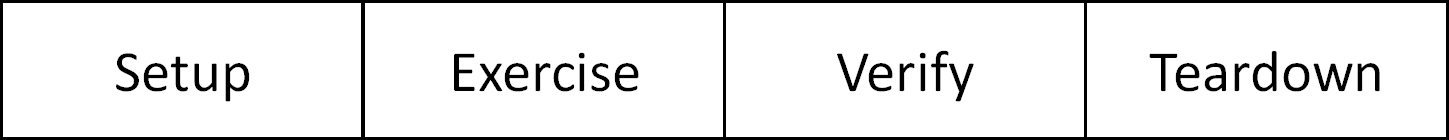
\includegraphics[width=0.95\columnwidth]{img/organisation_test.png}
            \caption{Code organization within a single test method }
            \label{fig:TestMethodOrganization}
        \end{figure}

        The \textbf{setup} component (also called fixture) sets up the required state to run the test. It instantiates objects (including the SUT and DOCs),
        initializes their internal state and creates
        the required connections between different objects. However, it only performs the minimum work needed to run the test.

        The \textbf{exercise} part executes the code that should be tested. In case of unit tests, this is often just a single line of code that only calls one method on the SUT.

        Afterwards, the \textbf{verify} code checks the test result and if everything worked correctly. This section decides it the test succeeded or failed using assertions.

        The \textbf{teardown} component cleans up behind the test. It closes open handles (file handles and database connections)
        and frees previously created memory if the language does not provide a garbage collector.

    \subsection{Test Classes and Suites} \label{subsec:TestclassesAndSuites}
        Each test method only tests one very small aspect of the SUT. The whole SUT functionality should be split up in as many test methods as possible to avoid big,
        confusing test methods that have to be refactored in every code change of the SUT. It also ensures easy defect localization \cite[p.~154]{Meszaros:2006:XTP:1076526}.
        This leads to many test methods even in small projects and requires further structuring into test classes and so called test suites (see \fref{fig:TestClassAndSuiteOrganization}).

        \begin{figure}[hbtp]
            \centering
            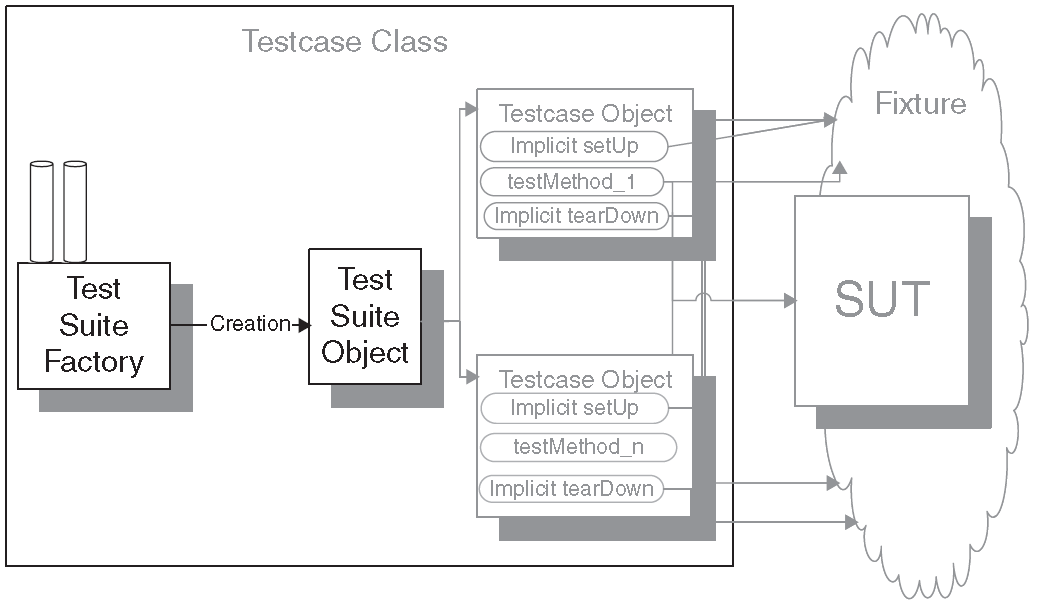
\includegraphics[width=\columnwidth]{img/organisation_big.png}
            \caption{Code organization: suites and classes \\ \cite[Chapter 24]{Meszaros:2006:XTP:1076526}}
            \label{fig:TestClassAndSuiteOrganization}
        \end{figure}

        A test class consists of multiple test methods, each with its individual setup and teardown components.
        There are different approaches to structuring tests into classes:

        \begin{itemize}
            \item \textbf{Test case Class per Class}
                    is a very common approach that ensures that test case classes do not grow too big and that tests and their associated SUT can be located easily.
            \item \textbf{Test case Class per Feature}
                    makes it easy to identify broken features.
            \item \textbf{Test case Class per Fixture}
                    reduces the test code and makes the test classes more readable (only a single \code{setup()} method is needed).
                    When using this technique, methods that require the same fixture (the same state before executing) are composited.
                    However, this approach can easily result in scattering test conditions across many test classes.
        \end{itemize}

        Testing frameworks automatically create a test suite that contains all existing test classes. In order to run the tests, the all-tests test suite can be executed.
        In smaller projects, dividing all test methods into test classes is usually enough.
        However, as soon as the project grows, the execution time of test methods starts playing an important role.
        Each code change (even a small one) requires the developer to execute the complete test suite, including all test methods ever written.
        To avoid this, test classes can be further divided into so called test suites.

        A test suite has a speaking name and is a collection of tests that belong together.
        Testing frameworks which support suites (like the xUnit family) allow classes to provide a test suite factory which returns a test suite.
        These factory methods create a new test suite object and attach other test suites, test classes or only single test methods to it.
        This allows developers to structure tests arbitrarily and only execute parts of the tests.



% ##############################################################################################################
% ##########   G E N E R A L
% ##############################################################################################################
\section{Terminology and Common Patterns} \label{sec:TerminologyAndPatterns}

    % ############################################################################################################ %
    \subsection{Fixture Setup Patterns} \label{subsec:FixtureSetupPatterns}
        Test fixtures are used to set up the required state for running a test.
        Test fixtures instantiate and initialize the SUT as well as DOCs and are also responsible for preparing test doubles \see{subsec:TestDoublePatterns}.

       Two kinds of fixtures exist:
        \begin{itemize}
            \item \textbf{Fresh fixtures}
                    are part of the test method itself. They are not reused in other test methods and are teared down at the end of the test.
            \item \textbf{Shared fixtures}
                    are constructed to be used in multiple test methods.
                    These methods can either be called once for all tests (the test state is reused),
                    or are automatically called before each test method (test code reuse).
                    The former is especially useful for building expensive objects like in-memory databases.
        \end{itemize}

        \fref{fig:TestOrganisationOfFixtures} illustrates the different locations where fixtures and their corresponding teardown routines are located.

        \begin{figure}[hbtp]
            \centering
            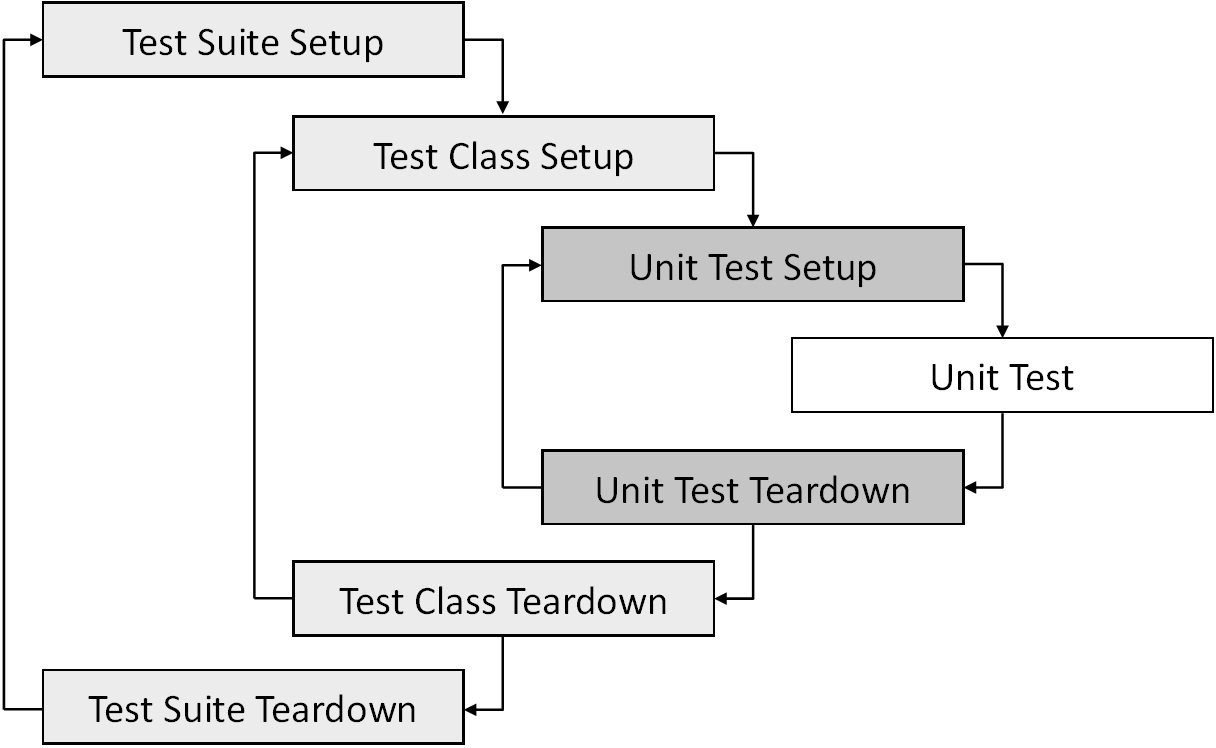
\includegraphics[width=0.9\columnwidth]{img/organisation_tests.jpg}
            \caption{Location of fixtures and their corresponding teardown routines. The dark gray components are fresh fixtures, while the light gray routines are shared fixtures and therefore reused between multiple unit tests.}
            \label{fig:TestOrganisationOfFixtures}
        \end{figure}

        \subsubsection{Fresh Fixture Setup}
            \begin{itemize}
                \item \textbf{In-line setup}
                        means that the constructor of the required objects (for example the SUT) is called directly within the test method.
                \item \textbf{Delegated setup}
                        facilitates creation methods that are responsible for returning usable objects.
                \item \textbf{Creation methods}
                        are used if the construction of objects is more complex.
                        For the test method itself it is unimportant how to construct such objects. To avoid unnecessary complexity, the code is moved to a separate method.
                \item \textbf{Implicit setup}
                        are \code{setUp()} routines in the test class (or test suite) that are automatically called by the testing framework.
            \end{itemize}


        \subsubsection{Shared Fixture Setup}
            \begin{itemize}
                \item \textbf{Prebuild fixtures}
                        are created implicitly by the testing framework before the first test is executed. They are usually located in the \code{setUp()} code of the test suite.
                        This is useful for objects that are expensive to build (time consuming) like in-memory databases.
                        Such objects are built only once and then reused by all tests. To avoid building the object for each test case, a singleton pattern can be utilized.
                \item \textbf{Lazy setup}
                        is similar to the prebuild fixture with one key difference: the object is not build in advance, but instead when the first test method tries to access it.
                        This can easily be implemented using a lazy initialized singleton but can lead to problems regarding the teardown execution, in which case the next strategy can be used:
                \item \textbf{Setup decorators}
                        are wrapped around the test suite, containing a decorator that executes code before and after the execution of all contained tests.
                \item \textbf{Suite fixture setup}
                        are the \code{setUp()} and \code{teadDown()} routines within the test suite.
                \item \textbf{Chained tests}
                        reuse the fixtures that are left over from the previous test method.
                        This is very similar to how a human tester tests code: while performing a long series of actions, the outcome of each intermediate step is verified.
            \end{itemize}

    % ############################################################################################################ %
    \subsection{Result Verification Patterns} \label{subsec:ResultVerificationPatterns}
        There are two different kinds of verification strategies:
        \begin{itemize}
            \item \textbf{State verification}
                    is the phrase if the SUT's internal state or the state of a DOC is verified after execution.
            \item \textbf{Behavior verification}
                    is the solution if there exists no state that can be checked.
                    In such a situation, the behavior on how the SUT interacts with its environment has to be evaluated.
                    Usually this requires the use of test doubles as described in chapter \ref{subsec:TestDoublePatterns}, p.~\pageref{subsec:TestDoublePatterns}.
        \end{itemize}

        \subsubsection{Assertion Method Styles}
            Depending on how assertions are used in test methods, different terminology is used to describe them.
            The following list contains some well-known terms for different assertion types.

            \begin{itemize}
                \item \textbf{Unfinished test assertions}\\
                        A common approach in writing tests is to first think about all required test cases and writing down the methods without implementation code.
                        Until the methods have been fully implemented, an \textit{unfinished test assertion} is used to force a test failure.
                        This kind of assertion is used to ensure that the developer does not forget to finish all test cases.
                \item \textbf{Custom assertions}\\
                        There is often a need for test-specific object comparisons that are reused in multiple test methods. In such cases, assertions are moved into 
                        a separate method to reduce duplicate code. 
                        Therefore, \textit{custom assertions} are needed if multiple assertions should be condensed into a single method (assertion) call.
                \item \textbf{Delta assertions}\\
                        These kind of assertions are often needed in case of shared fixtures (and therefore shared objects) 
                        that lead to tests influencing other tests. In such scenarios, the initial state of a test case can be different depending on which tests were executed beforehand.

                        Delta assertions take two separate state snapshots, one before and one after test execution, and compare them afterwards.
                        An example can be the number of database rows that have been inserted into a table.
                \item \textbf{Guard assertions}\\
                        An important principle of writing tests is to avoid conditional test logic. 
                        Conditional test logic are \code{if}s which are used to skip assertions, a scenario that should never happen in well-written test methods. 
                        Conditional test logic is a great sign of code smell which shows that something is wrong.

                        Sometimes, assertions must not be called since they would cause an error, like accessing an invalid object that solely exists because the SUT already failed the test.
                        In these situations, \textit{guard assertions} are used instead of \code{if}s to detect test failures and to abort test method execution before the dangerous assertions can be executed. 
                        Guard assertions can usually be found between the SUT execution phase and the verify phase. 
                \item \textbf{Shared fixture state assertions}\\
                        In case of shared fixtures, guard assertions can also be used at the beginning of a test to ensure that the fixture satisfies the test's needs.
                        These guard assertions are called \textit{shared fixture state assertions}.
            \end{itemize}

    % ############################################################################################################ %
    \subsection{Fixture Teardown Patterns} \label{subsec:FixtureTeardownPatterns}
        Fixture teardown is the process of closing open handles, unregistering events and freeing allocated memory.
        In languages like Java, the \textbf{garbage collected teardown} is able to do most of the work.

        Other languages like C++ use \textbf{automated teardowns} where the allocated memory has to be freed manually.
        This can be difficult because the developer has to provide a clean teardown for all possible outcomes, even if the test failed and the SUT is in an invalid state.

        Similar to the fixture setup \see{subsec:FixtureSetupPatterns}, the code organization of teardown logic distinguishes between \textbf{in-line teardown}, \textbf{delegated teardown}, \textbf{teardown methods} and \textbf{implicit teardown}.
        
 

    % ############################################################################################################ %
    \subsection{Test Double Patterns} \label{subsec:TestDoublePatterns}
        Test doubles are needed if the SUT depends on code that is cannot be included in the test.
        In these situations, the DOC has to be replaced by a so called \textit{test double} \cite{NirajBhattBlog:TestDoubles}.

        \begin{itemize}
            \item \textbf{Dummy objects}
                    are the simplest approach and just act as a simple placeholder without containing any logic. 
                    The most basic forms of dummy objects are a null-object or passing a \code{new Object()}.
            \item \textbf{Fake objects}
                    are very similar to stubs and often hard to distinguish. They implement the real object in the simplest way.
                    An example for a fake object is a database access double that always returns the same, hard-coded row and does nothing if new data should be inserted.
            \item \textbf{Stubs}
                    are influencing the SUTs to force specific code paths to be executed.
                    It is often possible to tell the stub in the fixture which code paths the SUT should execute.
                    In contrast to fake objects, stubs are trying to challenge the SUT by influencing it.
            \item \textbf{Spy objects}
                    provide values for the SUT like test stubs. But in addition to that, they also capture and save the input for later verification of the test.
                    Test spies are therefore very usable for behavior verifications \see{subsec:ResultVerificationPatterns}.
            \item \textbf{Mock}
                    objects are similar to test spies, with the difference that they are verifying the observed input while being executed instead of saving it for later.
        \end{itemize}

        Another distinction of test doubles is their construction:
        \begin{itemize}
            \item \textbf{Hard coded test doubles}
                    are created once and behave the same way in every situation.
            \item \textbf{Configurable test doubles}
                    are set up and configured in the fixture and can behave differently for different test methods which makes them more versatile and helps to reduce test code.
        \end{itemize}


        \fref{fig:TestDoubleRelations} illustrates the connections between the different test double types.

        \begin{figure}[hbtp]
            \centering
            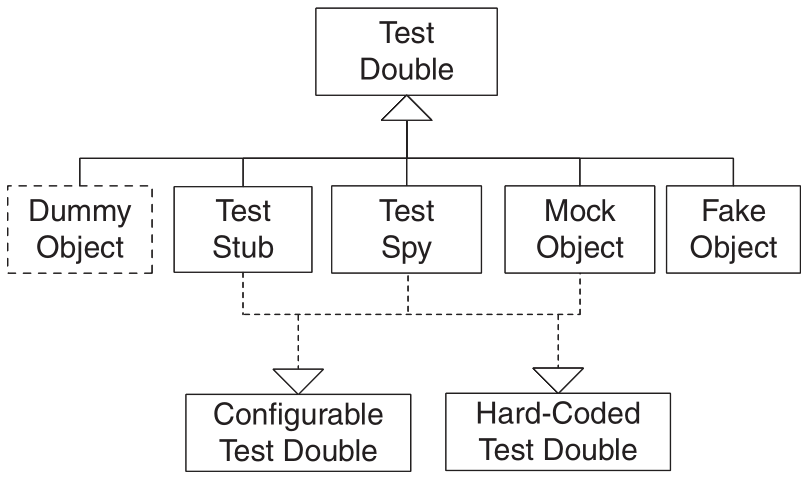
\includegraphics[width=\columnwidth]{img/testDoubles.png}
            \caption{Relations between different kinds of test doubles \cite[p.~527]{Meszaros:2006:XTP:1076526}.}
            \label{fig:TestDoubleRelations}
        \end{figure}




% ##############################################################################################################
% ##########   F . I . R . S . T .
% ##############################################################################################################
\section{F.I.R.S.T.} \label{sec:First}

    In order to have useful and maintainable code, test code should follow the same guidelines as production code
    and a dual standard should be avoided. 
    For more information about clean test code and clean code in general, see \cite[]{Martin:2008:CCH:1388398}.

    In addition to general coding guidelines, test code has five additional rules (F.I.R.S.T) to be considered as clean:

    \begin{itemize}
        \item \textbf{Fast}\\
                Tests should be run frequently to find problems as soon as possible, which requires them to run slowly.
                Tests that run slow cannot be executed after each change and problems are therefore detected late.  
        \item \textbf{Independent}\\
                Test cases should be independent from each other. It must be possible to run the tests in an arbitrary
                order or even simultaneously using multi-threading. If tests depend on other tests, the first failing
                test will cause a cascade of further failures, hiding actual problems in all those dependent unit tests.
        \item \textbf{Repeatable}\\
                Tests should work the same way on every environment and must always be deterministic. If a test requires
                a specific testing environment to run (for example an active network connection or stable database), there
                will always be an excuse for failing tests, making them pointless.
        \item \textbf{Self-Validating}\\
                A test always returns a boolean: Either the test failed, or it succeeded. It should never be necessary
                to manually check the result for its success, for example by examining the console output for specific log
                statements. 
        \item \textbf{Timely}\\
                Unit tests should be written just before the production code (TDD: test driven development). If tests are written
                after the production code has been finished, chances are high that they will never be written.
                Furthermore, if the production code is written first, it is possible that the written code is impossible to test,
                for example due to non-replaceable dependencies like system calls.
                This cannot happen if the tests are written beforehand.
    \end{itemize}


% ##############################################################################################################
% ##########   G E N E R A L
% ##############################################################################################################
\section{Test driven Game Development (TDGD)} \label{sec:TDGD}
    \fref{fig:GameDevLifeCylce}  shows the life cycle of  a game development project which usually consists of four different parts.

    \begin{figure}[hbtp]
        \centering
        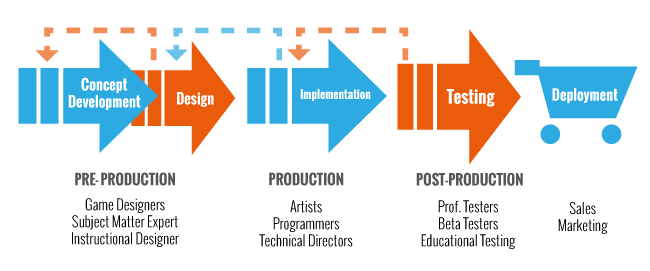
\includegraphics[width=0.95\columnwidth]{img/devCycle.png}
        \caption{Game development life cycle}
        \label{fig:GameDevLifeCylce}
    \end{figure}

    Historically, game testing is performed in the last phase, the ``post-production'' phase, where both professional testers as well as beta testers 
    are performing manual game testing by playing the game for many hours.
    Since automated testing got more and more popular 
    in the last few years, the game engineering sector also experienced major changes in regard to automated software testing
    and started to adapt agile ideas. 

    Thanks to many blogs like Noel Llopis's \cite[]{noel:testingBlog} there are indicators on how well TDD is acknowledged in the games industry. He addresses the fears and misconceptions that teams have about TDD. It can definitely be applied to games too. He points out numerous times that TDD is a guide to design the code base and that it is a development methodology. Francesco Carucci's presentation \cite{crytek:aaatesting} on Testing in AAA games goes in the same direction. Actually it goes one step further and states that using TDD lowers production costs because the time spent on debugging and maintaining the code can be reduced drastically. He points to a chart published at gamasutra \cite{gamasutra:automatedTests}. It shows the development phase of the Vision engine. They aggregated the bug reports and put the numbers of unit tests they had in their code base in the chart to put it into perspective. They stated that in the beginning they relied completely on manual test and even though every new version had been checked, the bug reports kept coming in.  
        \begin{figure}[hbtp]
        \centering
        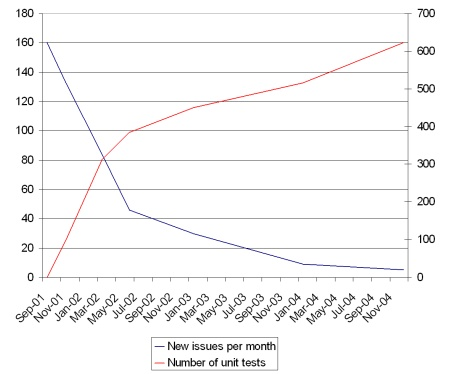
\includegraphics[width=0.95\columnwidth]{img/unittestissues.jpg}
        \caption{Describes the bug report / unit test curve for the Vision engine.}
        \label{fig:BugReportRatio}
    \end{figure}
    Many articles emphasize the fact that a fully automated continuous integration system is a key part to success, when quality code matters. These systems have to fulfill every task from build, deploy to automated testing with bug reports on errors. 
    \\ \\
    Although many articles argue that TDD should be used, they are not in complete agreement on what can and should be tested. First of all it needs to be pointed out that many articles are quite old and the more recent ones claim that almost everything can be tested. They also provide some guidelines on how to write the code testable:
    \begin{itemize}
        \item Keep the code as simple as possible
        \item Look for modularity
        \item Have low dependencies
        \item Avoid complicated states in objects
        \item Keep tests independent from each other
        \item Keep tests very fast
        \item Remove randomness from tests
    \end{itemize}
    Some side effects are that you can use the unit tests as documentation, because every comment needs to be maintained and the compiler cannot check if you updated your comments according to your refactoring.
    But with unit tests, you have at least one example of how to use the API in a correct way. Another benefit is that you always have a check that what you implemented is what you meant the code to do. There is almost instant feedback. If you fail a test you know where to fix the broken code. You also have the advantage to test your code on different platforms as your build server checks them for you. 
    \\ \\
    While it was discouraged to test things like graphic API calls or high level code in the past, it is now a normal thing to do. Llopis describes the way they approached it. For him there are three possible ways:
    \begin{itemize}
        \item Insert a layer between the graphics renderer and the graphics API. That way every call can be intercepted, checked for errors and - most important - unit tested. 
        \item Check for the API state. After every draw call the API is queried for the correct state. This approach has proven to be difficult because everything that has been altered needs to be cleaned up again. It also depends on the graphic API you want to use.
        \item Isolate graphic calls. This can be done if the other two options fail. 
            That gives the advantage that every call to that external API goes through one single point and can be tested to some extent, but does not give a lot more information about the call. That shouldn't be a problem since the own code should be tested and not the API.
    \end{itemize}


    \subsection{Tests during Game Development}
        The following section gives some examples for tests that can be easily utilized during game development.

        \begin{itemize}
            \item \textbf{Smoke testing} \\
                    These kinds of tests can be easily performed using an automatic test exerciser.
                    They usually focus on user interface logic (button clicking, menu opening, touch gestures)
                    and don't require very sophisticated test logic. 
                    Although smoke tests don't provide very detailed results, they are still very powerful in
                    finding simple flaws and providing quick feedback after code changes. 
            \item \textbf{Functional testing} \\
                    This is probably the single most important test group.
                    Functional tests check that the game behaves correctly and are usually associated with manual testing and playing the ``game through''. 
                    A common approach to deal with this kind of testing is to write an AI that automatically plays the game at a much higher speed than any human player.
                    This AI performs predefined actions and checks if the game responds as expected.
                    With such a test, developers can avoid game-breaking bugs like unsolvable levels and unbeatable enemies due to malfunctioning game elements.
                    If the AI is able to finish the level with a set of predefined actions, a human player should be able to do so too. 
            \item \textbf{Regression testing} \\
                    Regression tests are usually run after every code change and therefore before any commit.
                    They ensure that existing functionality is still working correctly after new features have been added.
                    It is important to note that regression tests should be performed regularly on all supported platforms to
                    ensure a certain level of confidence. 
                    The tests should also be extended after new functionality has been added.
            \item \textbf{Performance testing} \\
                    Most game engines already provide tools for performance testing and debugging, so it should be
                    easy to utilize this information and verify the differences in performance after a new feature has been added.
                    Performance testing can also give hints about other aspects of the game like battery consumption - an important aspect for mobile games.
            \item \textbf{Connectivity testing} \\
                    Most games today utilize some sort of network connectivity. They have server-client interaction, login checks,
                    social media features or just the ability to download additional game content while playing.
                    Connectivity tests ensure that the network communication is working correctly and not only involve game code, but also
                    server-side code that can be written in a completely different language. 
                    This kind of tests is also very important for anti-cheating functionality and security concerns.
            \item \textbf{Localisation tests} \\
                    These kinds of tests become important as soon as the game should be released on a global basis.
                    Localisation tests mainly test different translations on different platforms and ensure that GUI-layouts don't brake by comparing screen shots.
        \end{itemize}
        \cite[]{testdroid:agileProcess}.

        Last but not least the TDD way allows a company to stay agile and cope with change requests much more easy than without. 
        \fref{fig:CostOfChange} shows how difficult it would be if everything were implemented the traditional way and testing would take place in the post-production phase only.
        \begin{figure}[hbtp]
            \centering
            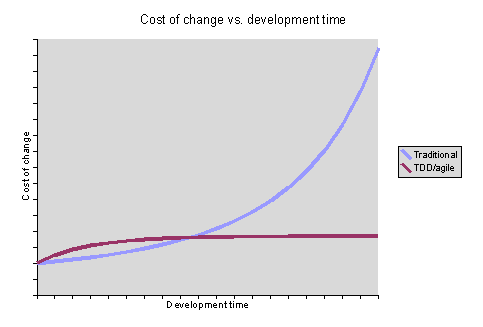
\includegraphics[width=0.95\columnwidth]{img/costofchange.png}
            \caption{Cost of change over development time.}
            \label{fig:CostOfChange}
        \end{figure}

% ##############################################################################################################
% ##########   N A N A N A N A N A   -   B A T M A N !
% ##############################################################################################################
\section{Case Example: Google} \label{sec:TestingAtGoogle}
    This chapter describes how testing is done at Google. For this paper the book ``How Google tests software'' \cite[]{whittaker2012google} has been chosen. It may be less important for testing in games itself, but could become a handy tool for testing server applications.
    Also, the book that was chosen for reference describes not only how it is done technically but also how the whole company utilizes testers to ship quality code in quick iterations. 
    The approach Google takes is called the \textit{quality first approach}. 
    The author says that the statement ``quality cannot be tested'' is wrong. He insists that the work flow should always be to write some code and then test this code with its according test. It is much more important to have a feature implemented rock solid rather than writing new ones. Google has also put some thought into the company's structure and how to combine it with testers that are not assigned to a certain division. First of all tests have to be implemented by the developers that write the code in the first place, simply for the reason that the author of the code should most likely spot the bug or take the least time to debug the code. 

    Quality can only be achieved if testing is an unavoidable aspect of the development. That is enforced not only through the company's structure but also through its code repository. Google defines different roles for different aspects of testing:
    \begin{itemize}
        \item \textbf{The software engineer (SWE) } does the usual coding in TDD but with a focus on features. He also does the majority of feature implementations.
        \item \textbf{The software engineer in test (SET)} is also a developer but is more the one that has to keep an eye on quality. He reviews code and improves it to be easier to maintain and to test. Not only does he improve the testability, he also provides the test infrastructure. 
        \item \textbf{The test engineer (TE)} is related to the SET role but has a different focus. He tests from the users perspective and not the developers perspective. His job is to write automation scripts that mimic users, he provides scenarios and he interprets the executed test and the result. 
    \end{itemize}
    These testing roles are part of a horizontally structured department. Its members work on all the projects and report to their own executive. 
    Every tester can raise any kind of concern, whether it is that there are too many bugs or a security problem. If a development team wants to take any kind of shortcuts like releasing a new version with fewer tests or the like, this has to be negotiated with the testing department. 

    Google always aims to release a new build as quickly as possible with some limitations. 
    The reason they want to get to the costumers as quickly as possible is that they need the feedback quickly. 
    If a brand new product is developed, they have a rule of thumb that the core product should be built and finished as fast as possible.
    As soon as the core is stable, it will be released so that a large group of people can be reached very early. 
    After that, the team has to iterate as fast as possible again and consider user feedback. 
    A thing to keep in mind though is that, just because it is an early version, it does not mean that it is bad or halfheartedly made.

    Google does not distinguish between \textbf{code}, \textbf{integration} and \textbf{system} testing. They name the tests after the scope size. Scopes can be:
    \begin{itemize}
        \item  \textbf{small} 
        \item  \textbf{medium}
        \item  \textbf{large}
    \end{itemize}

    The smaller a test, the more likely it is to be automated. Small tests cover only units of code, medium tests cover multiple units in a faked environment 
    and large tests cover any number of units in production environment and without (!) any faked resources. The coverage for each category has to be within acceptable limits.
    For example, if medium and large tests cover only a low percentage and small tests cover most of the system, the system probably has end to end user problems. 

    It is also important to note that tests should fulfill the following:
    \begin{itemize}
        \item  They are independent so they can be executed in any order.
        \item  They must not have any side effects.
        \item  They must not alter the environment or require any environment modifications.
    \end{itemize}

    A general rule of thumb to distinguish what should be tested automatically is whether it requires human intuition to test. 
    If it cannot be automated in the first place, the tests are recorded whenever possible and repeated by scripts or similar methods. 
    Very important in the whole testing process is that the section that leads to a test failure is pinned down 
    and the authors of the affected code are notified automatically. The system should also file a bug report with the authors tagged to it.

    It has already been mentioned that testing is a horizontally structured department at Google. 
    Therefore, it is not guaranteed that every project has testers of said department on board. Every project team has to request staff form this department. They have to convince the testers that their project is exciting and full of potential. 

    The basic work flow at Google is one of the following:
    \begin{enumerate}
        \item \textbf{Test planning} \\
        It is done with Google Test Analytics. It is risk-based, quick and automatically updated.
        \item \textbf{Test coverage} \\
        New versions are checked by bots for differences. If they find any differences, they are reported to humans for quick evaluation.
        \item \textbf{Bug evaluation} \\
        It is determined whether these differences are bugs or new features.
        \item \textbf{Exploratory testing} \\
        This is done by crowd testers and early adopters. These bugs are mostly related to configuration and context. These bugs are hard to spot and require human intelligence to induce and report.
        \item \textbf{Triage and debugging} \\
        Realtime dashboards provide an overview of bug trends. Bugs are reported with the data needed to investigate the problem.
        Usually there is also a recording on how to reproduce the bug in front of the developers' eyes.
        \item \textbf{Deploy and return to step 1.} \\
        Rinse and repeat.
    \end{enumerate}

    \begin{figure}[hbtp]
        \centering
        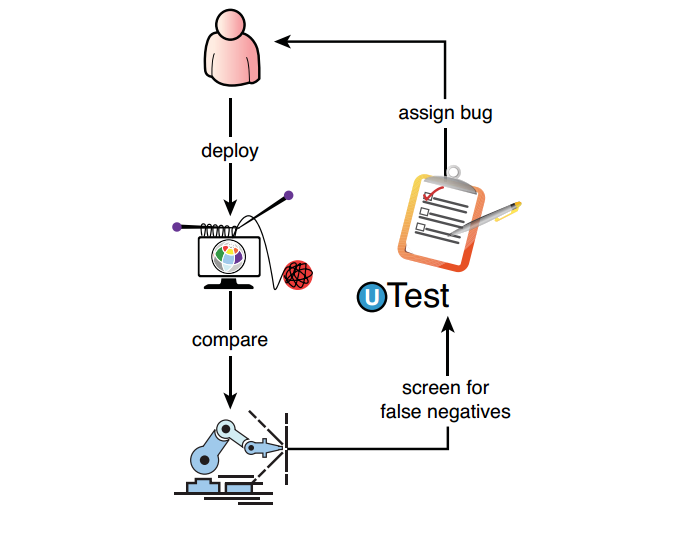
\includegraphics[width=0.95\columnwidth]{img/testingWorkflow.png}
        \caption{Workflow at Google}
        \label{fig:WorkflowAtGoogleTDD}
    \end{figure}

    Every engineer at Google can change his projects after a period of 18 months - if he wants to. 
    Therefore, it is a policy that dependencies on people should be avoided. This means that if there are rock star like developers in a team, 
    everything should be done to embody whatever this person is so good at into some tool or packaged in a way to be useful for others. 
    \\ \\ 
    One problem that arises is the following:
    When testing becomes a service that everyone can outsource to the testing department, 
    developers won't write the code to be easily tested.
    - Simply because they don't think about it while they are writing it. Therefore, quality and TDD has to become a mindset of any developer in the company.
    \\ \\
    Google's testing process in a quick overview: 
    \begin{itemize}
        \item Put quality in the work flow of every engineer.
        \item When done earnestly and honestly, quality increases.
        \item Freshly written code is better.
        \item Early builds are better.
        \item Integrations are unnecessary. System testing can concentrate on real user-oriented
            issues.
        \item Keep the projects and all the engineers free of accumulated bug debt.
    \end{itemize}

    \subsection{Applying Google's Approach to the Games Industry}
        It has been pointed out in the chapters before 
        that TDD is entering the games industry.
        It has definitely proven to be very important in other parts of the industry. 
        Many systems could not be created or operated without properly tested code. 
        As systems grow bigger and bigger, it is hard to keep track of everything necessary. 
        Even if it may be difficult to unit test games, in particular everything that appears only visual, 
        it might be a good advice that doing at least some testing is better than no testing. 
        
        What we can learn from Google's approach would be:
            Test whatever can be tested automatically and then go back to the tests where human interaction is necessary. Then you have to decide what can be scripted after recording and what has to be manually tested all the time. It may turn out to be very little that cannot be tested automatically after all.

% ##############################################################################################################
% ##########   G E N E R A L
% ##############################################################################################################
\section{Testing C++ with Google Test} \label{sec:GoogleTest}
A straight forward tool to write unit tests in C++ is gTest by Google. With its current version 1.7.1 some examples are implemented to be shown in this paper. 
There are different ways to setup a project but one thing that always has to be kept in mind is that test code should not be shipped. 
For that reason the project (VS: ``Solution'') is split in different parts. 
    \begin{enumerate}
        \item A DLL that houses all the code under test.
        \item The Google test project that uses the DLL and tests it. The test code is in this project.
        \item A thin client that produces the end result and contains code that will not be tested. This is usually built to an exe, utilizing functionality from the DLL.
    \end{enumerate}
    \begin{figure}[hbtp]
        \centering
        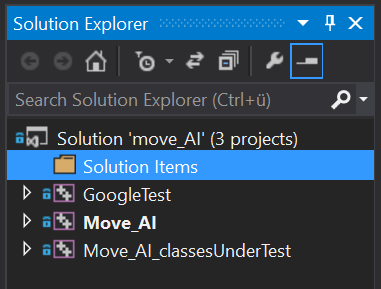
\includegraphics[width=0.7\columnwidth]{img/SolutionSetup.PNG}
        \caption{Solution setup in Visual Studio}
        \label{fig:SolutionSetup}
    \end{figure}

    \fref{fig:SolutionSetup} shows how the solution setup could look like. 
    It is also possible to have the main project house the test code and to stripe everything out on a Release Build with custom scripts. 
    To use gTest, it is only necessary to include it via Nuget or set it up the usual way via include paths in Visual Studio's project properties. 
    The main function for gTest can be seen in \fref{fig:gtestMain}. It only takes one include and one call to get everything running.
    
    \begin{figure}[hbtp]
        \centering
        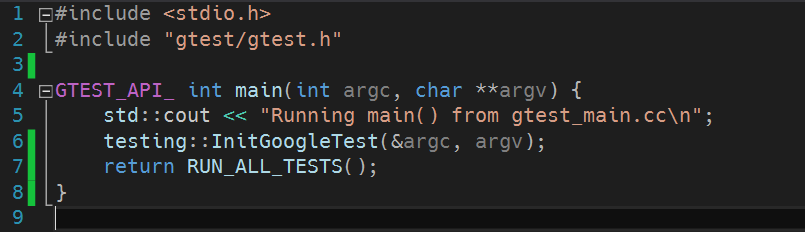
\includegraphics[width=\columnwidth]{img/gtestMain.PNG}
        \caption{Google test main}
        \label{fig:gtestMain}
    \end{figure}

    After that, every test in the gTest project is found automatically and will be called sequentially.
    There are also different ways to execute tests,
    one is building the gTest project into an exe and start it seperatly. This is also useful for continuous integration because it only requires MSBuild to be installed.
    An output example of this test runner can be seen in \fref{fig:gtestExe}. 
    Another option is to use Resharper as seen in \fref{fig:gtestResharper}.
   
    \begin{figure}[hbtp]
        \centering
        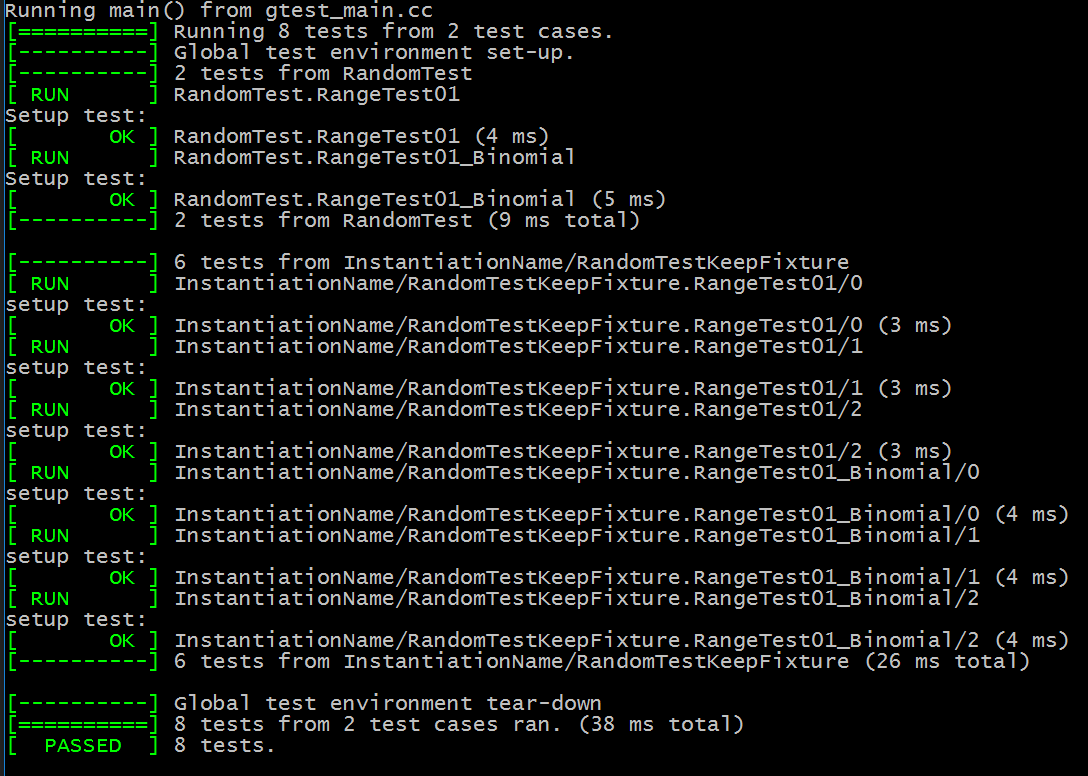
\includegraphics[width=\columnwidth]{img/gtestExe.PNG}
        \caption{Google test exe}
        \label{fig:gtestExe}
    \end{figure}
    \begin{figure}[hbtp]
        \centering
        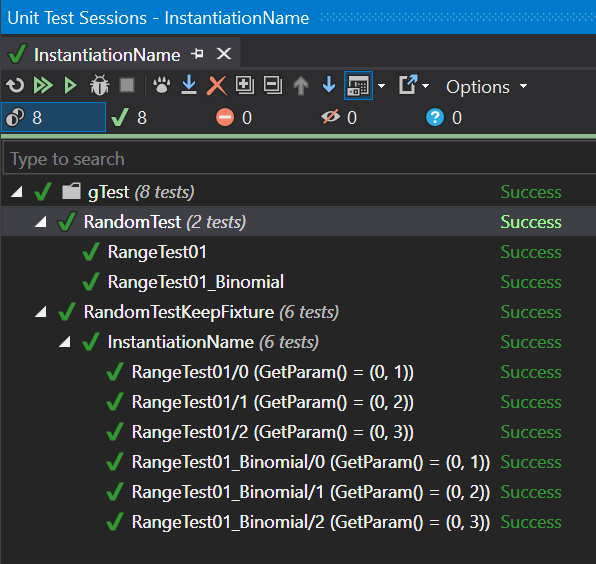
\includegraphics[width=0.8\columnwidth]{img/gTestResharper.PNG}
        \caption{Google test resharper}
        \label{fig:gtestResharper}
    \end{figure}

    Resharper allows the execution of every test individually. It can also run tests grouped together and is capable of debugging  test code really easily.
    Tests are written with some very basic defines. The most simple example might be shown in \fref{fig:gtestSimpleTest}.
    Tests are defined with the \code{TEST}-define, a test group name as well as a test name. Assertions are inserted with different variants of the \code{EXPECT} macro. 
    
    \begin{figure}[hbtp]
        \centering
        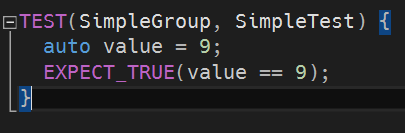
\includegraphics[width=0.6\columnwidth]{img/SimpleTest.PNG}
        \caption{Assertions in gTest}
        \label{fig:gtestSimpleTest}
    \end{figure}

    As soon as some state has to be set up for more that one test, fixtures become a handy tool. 
    To create one, the \code{Test} class has to be extended and is then provided as the first parameter for the \code{TEST\_F} defines. 
    \fref{fig:gtestFixture} shows an example.
    
    \begin{figure}[hbtp]
        \centering
        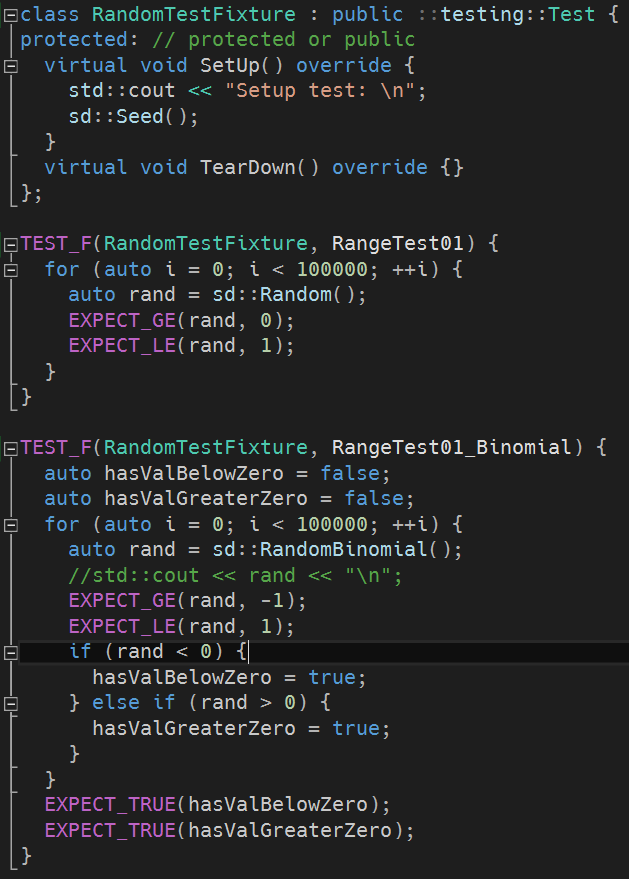
\includegraphics[width=0.8\columnwidth]{img/gtestFixture.PNG}
        \caption{Google test tests with a fixture}
        \label{fig:gtestFixture}
    \end{figure}

    Parameterized functions become useful as soon as the same functionality should be called with lots of different data.
    Parameterized tests are written like conventional tests with a fixture, with the difference that they are instantiated using the \code{INSTANTIATE\_TEST\_CASE\_P} macro.
    
    \begin{figure}[hbtp]
        \centering
        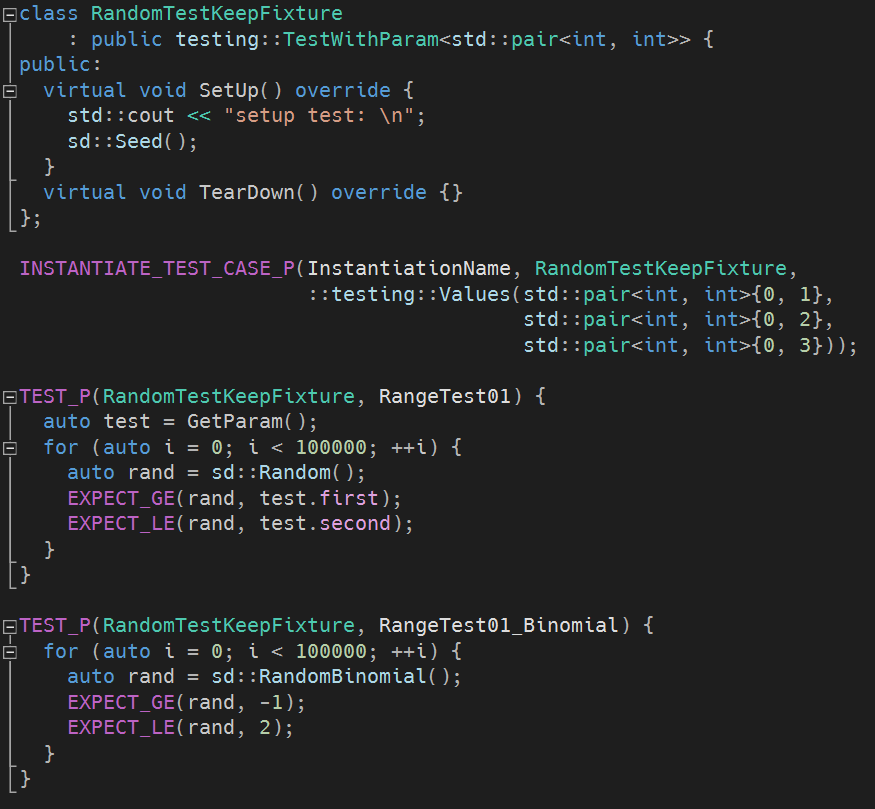
\includegraphics[width=\columnwidth]{img/gtestParam.PNG}
        \caption{Google test parametrized tests}
        \label{fig:gtestParam}
    \end{figure}

     \fref{fig:gtestParam} shows a simple example how parameterized tests look like.


% ##############################################################################################################
% ##########   G E N E R A L
% ##############################################################################################################
\section{Testing with Unity} \label{sec:Unity}
    As soon as Unity is used to develop a game project, ``Unity Test Tools'' is the way to go for implementing test cases.

    ``Unity Test Tools is a test framework for the games and interactive content you make in Unity. 
        By using these tools you can build quality products from the ground up. 
        Unity Test Tools are set up to feel like a natural extension of the Editor, 
        efficient and intuitive to use and they are free on the Asset Store.'' \cite[]{unity3d:TestToolsQA}

   % \subsection{Setup}
% TODO!
% ---

% ---
    \subsection{Integration Test Framework}
        Integration tests are designed to use a completely separate scene only for testing.
        This scene can be considered as a test suite \see{subsec:TestclassesAndSuites} and
        can continue multiple tests. Tests are executed one after another (not in parallel) to avoid mutual influences.

        \textbf{Test Execution Procedure} \label{unityIntTestExecOrder}
        \begin{enumerate}
            \setlength\itemsep{-0.4em}
            \item Play mode is enabled
            \item The first (or next) test object is activated
            \item Wait until test has finished or a timeout occurred
            \item Current active test gets deactivated
            \item If there are more tests, go to step 2
            \item Report results and finish test run
        \end{enumerate}

        Test objects are conventional GameObjects that have a TestComponent attached.
        Every GameObject that is under the hierarchy of the test object is considered to belong to this test only.
        Every other GameObject is common for every test on the scene.

        Note that test objects can also be nested to form test groups, in which case the parent test object is not executed as a discrete test.
        \fref{fig:UnityIntTestExample} shows an example of two test groups with seven tests, three of them failing and one configured to be ignored.

        \begin{figure}[hbtp]
            \centering
            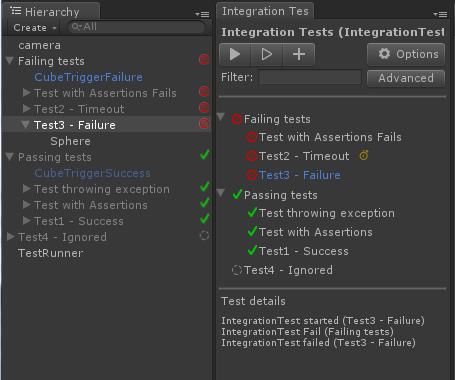
\includegraphics[width=\columnwidth]{img/unityIntegrationTestExample.png}
            \caption{Integration Tests with Unity Test Tools}
            \label{fig:UnityIntTestExample}
        \end{figure}

        \subsubsection{Manual Integration Tests}
            The easiest way to add tests to a Test Scene is by adding a Test Component to the desired GameObject.
            Every test component gets a reference to the associated test script and holds settings like the timeout or expected exceptions.
            An alternative is to use the Test Runner for adding new tests \see{subsubsec:UnityIntTestRunner}.
            However, these test objects can also be created automatically by using so called ``Dynamic Integration Tests''.

        \subsubsection{Dynamic Integration Tests}
            A more convenient way to add tests is to annotate the test scripts themselves from within the code.
            In order to mark a class as a test class, it has to derive from \code{MonoBehaviour} and contain the attribute
            \code{[IntegrationTest.DynamicTest (testSceneName)]} on top of it.
            The runner automatically discovers the new test class by using reflection and displays it on the list.  

            Other testing attributes can be added as well:
            \begin{itemize}
                \setlength\itemsep{-0.4em}
                \item \code{[IntegrationTest.Ignore]}
                \item \code{[IntegrationTest.ExpectExceptions (false, typeof(ArgumentException))]}
                \item \code{[IntegrationTest.SucceedWithAssertions]}
                \item \code{[IntegrationTest.Timeout(1)]}
                \item \code{[IntegrationTest.ExcludePlatform()]}
            \end{itemize}

            Tests are executed automatically as soon as the test object gets enabled \see{unityIntTestExecOrder}
            and can have different conditions to be stopped:
            \begin{itemize}
                \setlength\itemsep{-0.4em}
                \item \code{Testing.Pass()} gets called, the test succeeds.
                \item \code{Testing.Fail()} gets called, the test fails.
                \item The timeout is reached and the test gets aborted. It fails.
                \item An unknown exception gets thrown, the test fails.
                \item A known exception is thrown and the test passes.
                \item Every assertion component has been checked at least once.
            \end{itemize}

        \subsubsection{Integration Test Runner} \label{subsubsec:UnityIntTestRunner}
            Since Unity 5.3, the Test Runner became part of the Editor itself and was removed from the Unity Test Tools package.
            
            \fref{fig:UnityIntTestRunner} shows the Controls of the Test Runner within the Unity IDE:

            \begin{figure}[hbtp]
                \centering
                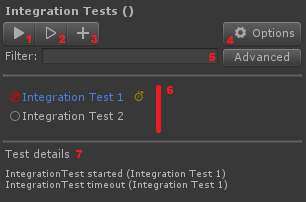
\includegraphics[width=\columnwidth]{img/UnityIntegrationTestRunner.png}
                \caption{The Unity Integration Tests Runner}
                \label{fig:UnityIntTestRunner}
            \end{figure}

            \begin{enumerate}
                \setlength\itemsep{-0.4em}
                \item Run all tests in the scene
                \item Run selected tests only
                \item Create a new test object
                \item Various test runner options
                \item Filter tests by name or state (succeeded, failed, ignored, ...)
                \item List all tests that are part of the scene
                \item Log messages and exceptions (test console)
            \end{enumerate}

        \subsubsection{Platform Runner} \label{subsubsec:UnityPlatformRunner}
            Unity also comes bundled with the ``Platform Runner'' which can be used to run the test scene(s) automatically on different platforms like Android.

            For more information on how to use Unity Test Tools, refer to their wiki at \cite[]{bitbucket:unityTestToolsWiki}.

    \subsection{Assertion Components}
        Assertion components are the second most important part of Unity Test Tools. They are used to assert desired states of game objects and decide if tests should pass or fail.
        Assertion components can be fully set up and configured using the GUI and consist out of a condition that must evaluate to true, as well as a timing component that defines when the condition should be checked.
        If a condition is not met, an exception is thrown in order to allow the investigation of the issue. 
        It is also possible to enable ``Error on pause'', which pauses the execution whenever an error occurs.

        \fref{fig:AssertionComponents} shows an example for such an Assertion Component. Note that is it also possible to write custom Assertion Components.


        \begin{figure}[hbtp]
            \centering
            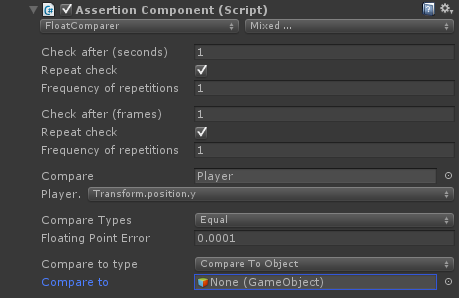
\includegraphics[width=0.95\columnwidth]{img/UnityAssertionComponent.png}
            \caption{Unity Assertion Components}
            \label{fig:AssertionComponents}
        \end{figure}

    \subsection{Continuous Integration}
        It is also possible to run the integration tests from within a command line without opening the Unity IDE:
\begin{lstlisting}
Unity.exe -batchmode -projectpath ...
    -executeMethod UnityTest.Batch.RunIntegrationTests
    -testscenes=TheScene
    -targetPlatform=StandaloneWindows
    -resultsFileDirectorty=Results
\end{lstlisting}

% TODO

% NSubstitute library
% NSubstitute is shipped with the Unity Test Framework. Please use its documentation for help: http://nsubstitute.github.io/help.html 




%===
%NSubstitue:
%    create mocks/spies easily from interfaces (without actually defining the implementation)


% ##############################################################################################################
% ##########   Conclusion
% ##############################################################################################################
\section{Conclusion}
As we have shown in this paper, testing is not only an important part in the software industry but also in the games industry. Certain rules and guidelines for testing are advantageous. These are described in the first part of the paper. The second part focuses on testing in real projects. Google's testing culture is described in greater detail. Also, their testing framework gTest is introduced. As a comparison we have also analyzed Unity's testing possibilities. This paper has shown that testing in games is definitely possible and should be done regardless of the size of the project.

% ##############################################################################################################
% ##########   A B B R E V I A T I O N S
% ##############################################################################################################
\section{Index of Abbreviations}
\begin{acronym}[XXXXX]
    \acro{DOC}[DOC]{dependent-on component}
    \acro{GUI}[GUI]{graphical user interface}
    \acro{SET}[SET]{software engineer in test}
    \acro{SUT}[SUT]{system under test}
    \acro{SWE}[SWE]{software engineer}
    \acro{TDD}[TDD]{test driven development}
    \acro{TDGD}[TDGD]{test driven game development}
    \acro{TE}[TE]{test engineer}
\end{acronym}

% ##############################################################################################################
% ##########   T H E   E N D
% ##############################################################################################################
%\bibliographystyle{apalike-url}
%\bibliography{Bibliography}
%
%\end{document}